%*****************************************
\chapter{Data}\label{06:data}
%*****************************************
%TODO Status: pre-draft

\begin{wrapfigure}{r}{0.4\textwidth}
	\label{06:fig01} 
	\centering
	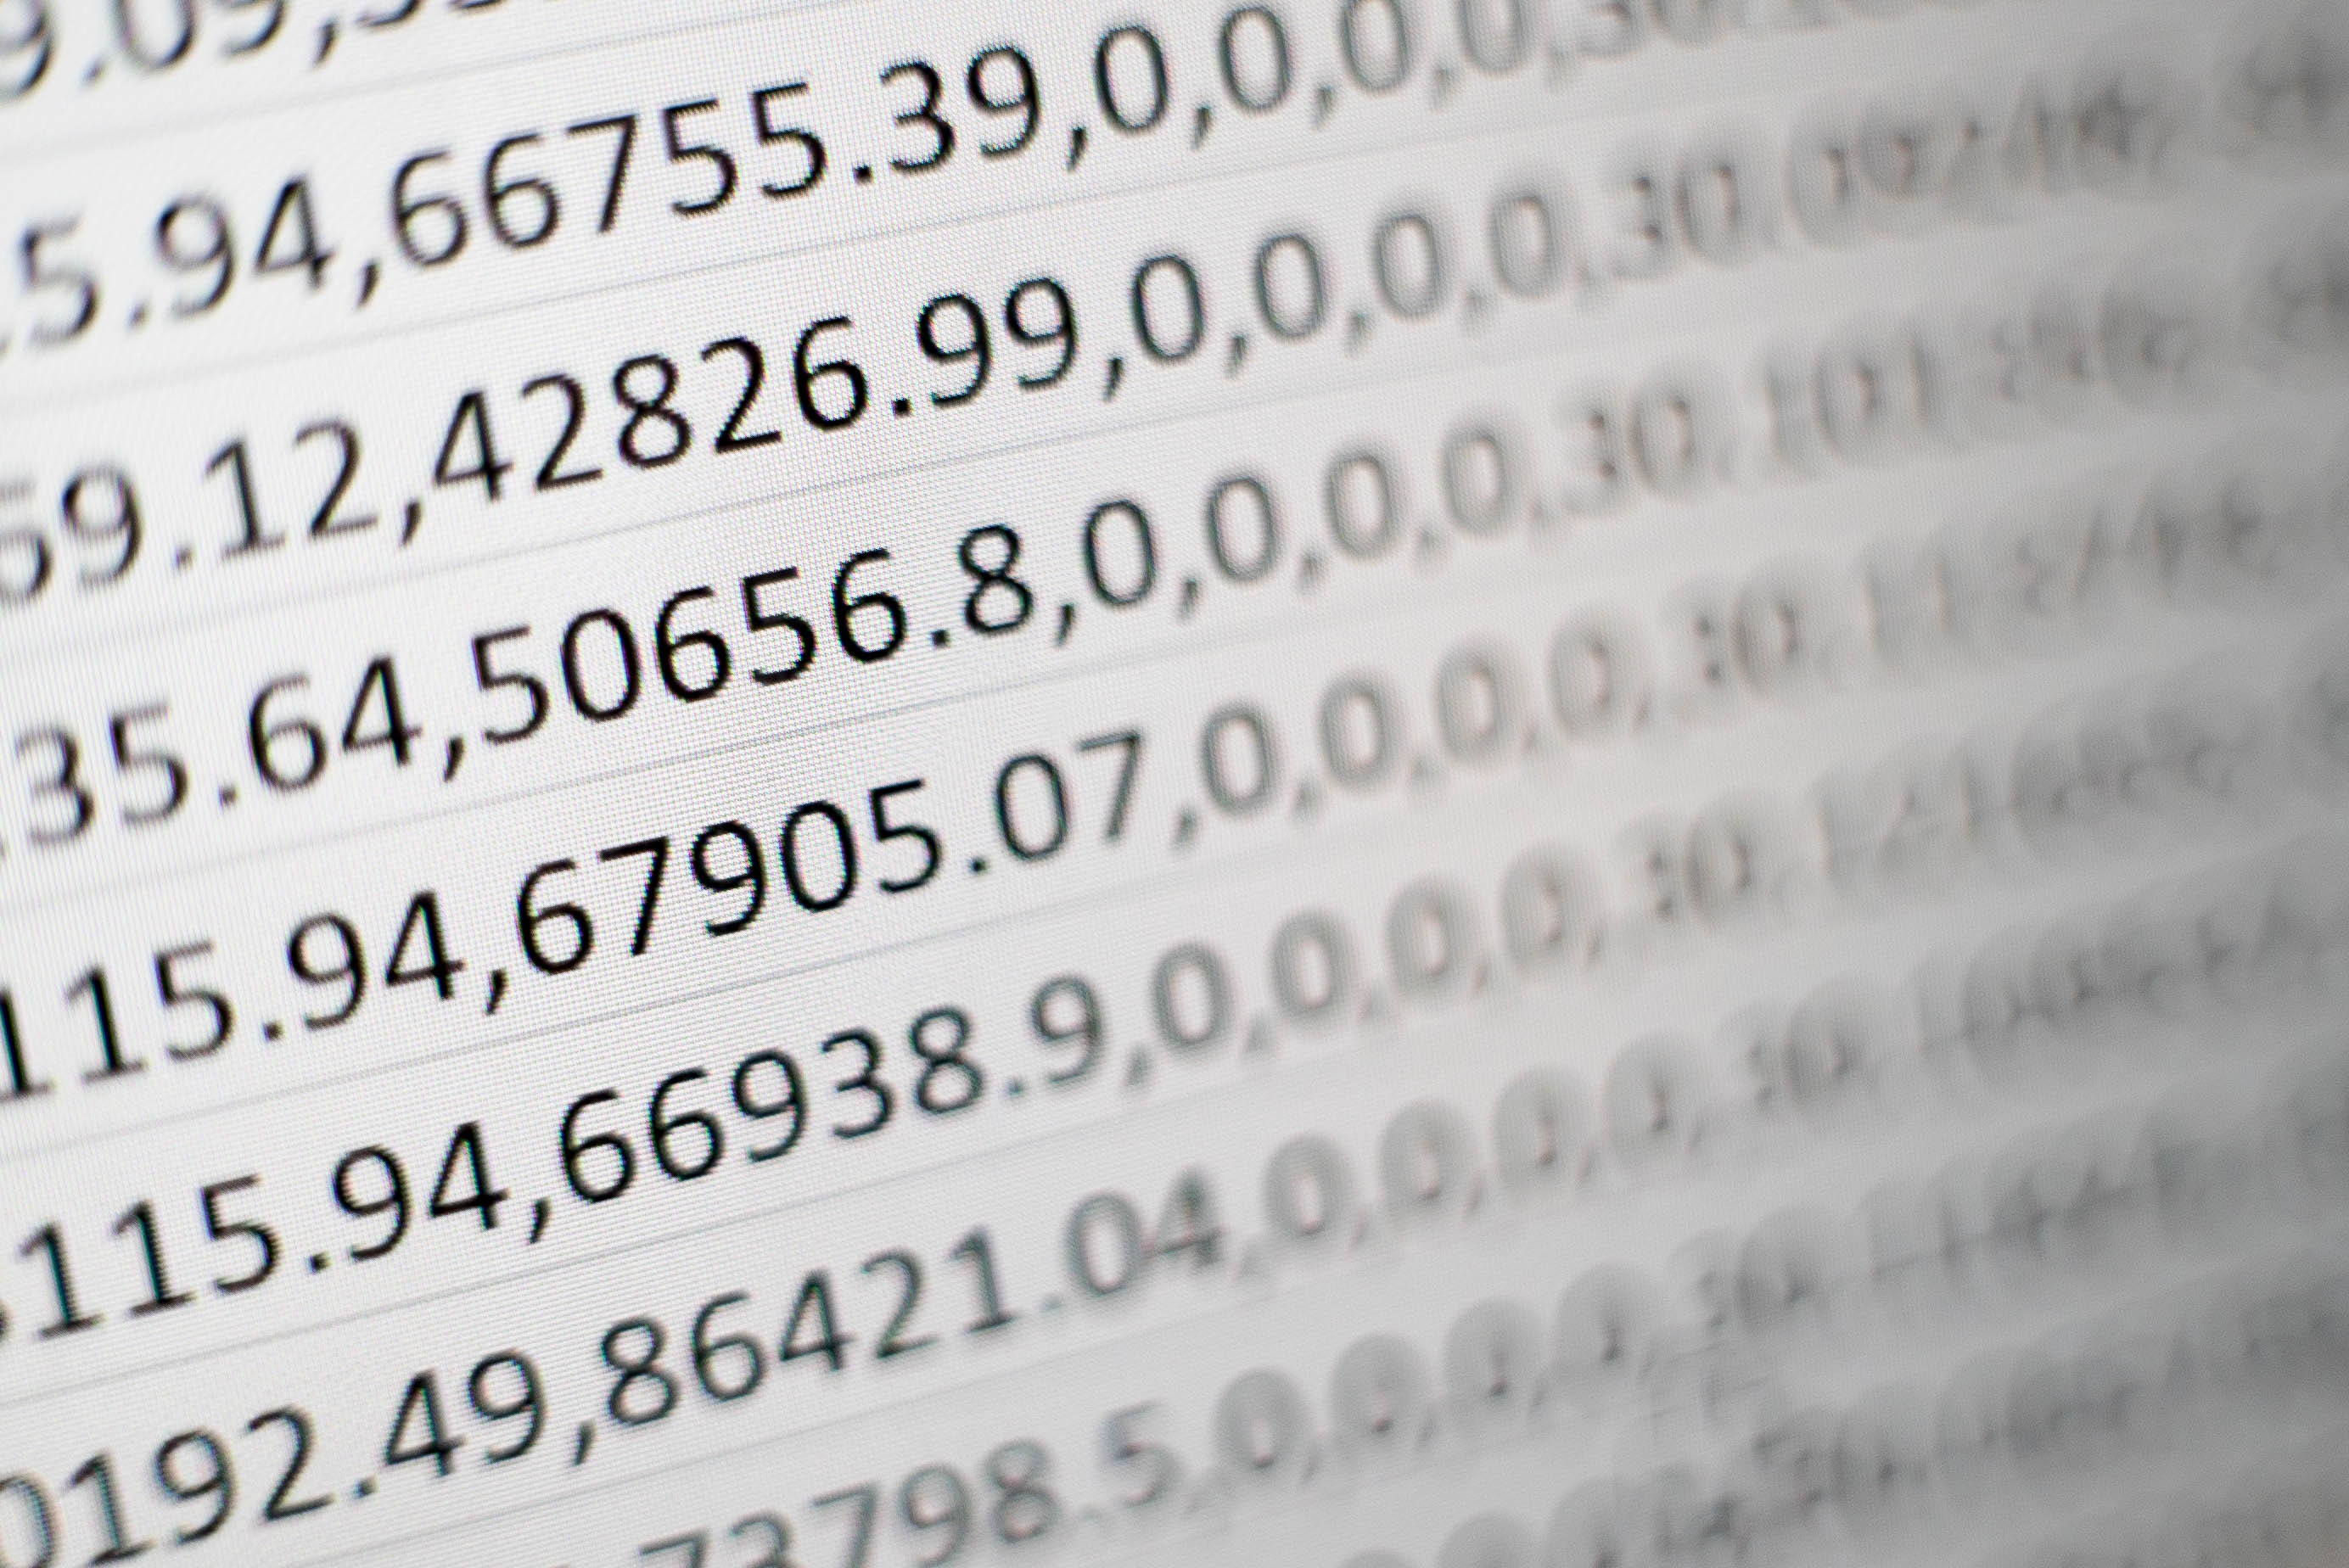
\includegraphics[width=0.4\textwidth]{gfx/06-data} 
\end{wrapfigure}
Data are\footnote{The word ``data'' is plural and is treated that way in this text even though modern usage seems to be trending toward a singular form.} a collection of facts about some topic. As examples, a ``customer loyalty'' program gathers data from customers on how often they shop, what they purchase on each trip, what time of day they typically shop, and all sorts of other data. When data are interpreted in some way they become information. The types of analyses that can be done with data are limited by the types of data involved. The purpose of this chapter is to introduce various concepts about data and show how they can be analyzed.\footnote{Photo by Mika Baumeister on Unsplash}


\subsection{Types of Data}

Psychologist Stanley Smith Stevens defined four generic types of data\cite{stevens1946theory}. 

\begin{itemize}
	
	\item \textbf{\Gls{qualitativedata}} groups observations into a limited number of categories; for example, type of pet (cat, dog, bird, etc.) or place of residence (Arizona, California, etc.). Because qualitative data do not have characteristics like means or standard deviations, they are analyzed using non-parametric tests, like Kruskal-Wallis H and Mann-Whitney U. Qualitative data can be further divided into two sub-types, nominal and ordinal.
	
	\begin{itemize}
		\item \textbf{\Gls{nominaldata}} are categories that do not overlap and have no meaningful order, they are merely labels for attributes. Examples of nominal data include occupations (custodial, accounting, sales, etc.) and blood type (A, B, AB, O). A special subcategory of nominal data is binary, or dichotomous, where there are only two possible responses, like ``yes'' and ``no''. Nominal data are sometimes stored in a database using numbers but they cannot be treated like numeric data. For example, binary data, like ``Do you rent or own your home?'' can be stored as ``1 = rent, 2 = own'' but the numbers in this case have no numeric significance and could be replaced by words like ``Rent'' and ``Own.''
		
		\item \textbf{\Gls{ordinaldata}} are categorical data but, unlike nominal, the categories imply some sort of order (which is why it is called ``ordinal'' data). One example of ordinal data is the ``star'' rating system for movies. It is clear that a five-star movie is somehow better than a four-star movie but there is no way to quantify the difference between those two categories. As another example, it is common for hospital staff members to ask patients to rate their pain level on a scale of one to ten. If a patient reports a pain level of ``seven'' but after some sort of treatment later reports a pain level of ``five'' then the pain has clearly decreased but it would be impossible to somehow quantify the exact difference in those two levels. Ordinal scales are most commonly used with Likert-type survey questions where the responses are selections like ``Strongly Agree'', ``Agree'', ``Neutral'', ``Disagree'', ``Strongly Disagree''. Ordinal data are also used when numeric data are grouped. For example, if a dataset included respondents' ages then those numbers could be grouped into categories like ``$ 20-29 $'' and ``$ 30-39 $.'' Those groups would typically be stored in the dataset as a single number so maybe ``$ 2 $'' would represent the ages ``$ 20-29 $,'' which would be ordinal data.
	\end{itemize}
	
	\item \textbf{\Gls{quantitativedata}} are numbers, typically counts or measures, like a person's age, a tree's height, or a truck's weight. Quantitative data are measured with scales that have equal divisions so the difference between any two values can be calculated. Quantitative data are discrete if they are represented by integers, like the count of words in a document, or continuous if they are represented by fractional numbers, like a person's height. Because quantitative data includes characteristics like means and standard deviations, they are analyzed using parametric tests, like T-tests and Analysis of Variance (ANOVA). Quantitative data can be further divided into two sub-types, interval and ratio.
	
	\begin{itemize}
		\item \textbf{\Gls{intervaldata}} use numbers to represent quantities where the distance between any two quantities can be calculated but there is no true zero point on the scale. One example is a temperature scale where the difference between $ 80 $\textdegree and $ 90 $\textdegree is the same as the difference between $ 60 $\textdegree and $ 70 $\textdegree. It is important to note that interval data do not include any sort of true zero point, thus zero degrees Celsius does not mean ``no temperature,'' and without a zero point it is not reasonable to make a statement like $ 20 $\textdegree is twice as hot as $ 10 $\textdegree.
		
		\item \textbf{\Gls{ratiodata}} use numbers to describe a specific measurable distance between two quantities; however, unlike interval data, ratio data have a true zero point. A good example of ratio data is the sales report for an automobile dealership. Because the data are a simple count of the number of automobiles sold it is possible to compare on month with another. Also, since the scale has a true zero point (it is possible to have zero sales) it is possible to state that one month had twice the sales of another.
	\end{itemize}
\end{itemize}

\section{Rating Scale}

When working with qualitative data, it is important for researchers to determine a rating scale, also called levels of measure, to record data gathered about any one attribute. For example, male-female-other, M-F-O, and $ 1 $-$ 2 $-$ 3 $ are three potential rating scales for the attribute \textit{gender}. A researcher could use any of these scales, or devise a completely different one, as long as the scale is used consistently throughout the entire research project. It is easy to imagine that many rating scales exist but the most common ones are \textit{binary}, \textit{Likert}, \textit{semantic differential}, and \textit{Guttman}. 

\begin{description}
	\item[\Gls{binaryscale}] Binary scales are nominal scales consisting of binary items that assume one of only two possible values, such as yes or no, true or false, and so on. For example, a typical binary scale for a ``political activism'' construct may consist of the six binary items shown in Table \ref{tab06.02}. Each item in this scale is a binary item, and the total number of ``yes'' indicated by a respondent (a value from $ 0 $ to $ 6 $) can be used as an overall measure of that person's political activism. Binary scales can also employ other values, such as male or female for gender, full-time or part-time for employment status, and so forth. If an employment status item is modified to allow for more than two possible values (e.g., unemployed, full-time, part-time, and retired), it is no longer binary, but still remains a nominal scaled item.
	
	\begin{table}[H]
		\centering
		\begin{tabularx}{0.95\linewidth}{p{0.70\linewidth}p{0.09\linewidth}p{0.09\linewidth}}
			\toprule
			\textbf{Question} & \textbf{Yes} & \textbf{No} \\
			\midrule
			Have you ever written a letter to a public official? & $ \bigcirc $ & $ \bigcirc $ \\ 
			Have you ever signed a political petition? & $ \bigcirc $ & $ \bigcirc $ \\ 
			Have you ever donated money to a political cause? & $ \bigcirc $ & $ \bigcirc $ \\ 
			Have you ever donated money to a candidate running for public office? & $ \bigcirc $ & $ \bigcirc $ \\ 
			Have your ever written a political letter to the editor of a newspaper?& $ \bigcirc $ & $ \bigcirc $ \\ 
			Have you ever persuaded someone to change his/her voting plans? & $ \bigcirc $ & $ \bigcirc $ \\ 
			\bottomrule
		\end{tabularx}
		\caption{Political activism binary scale}
		\label{tab06.02}
	\end{table}
	
	\item[\Gls{likertscale}] Designed by Rensis Likert, this is a very popular rating scale for measuring ordinal data in business research. This scale includes Likert items that are simply-worded statements to which respondents can indicate their extent of agreement or disagreement on a five or seven-point scale ranging from ``strongly disagree'' to ``strongly agree.'' A typical example of a six-item Likert scale for the ``employment self-esteem'' construct is shown in table \ref{tab06.03}. Likert scales are summated scales, that is, the overall scale score may be a summation of the attribute values of each item as selected by a respondent.
	
	\begin{table}[H]
		\centering
		\begin{tabularx}{0.95\linewidth}{p{0.35\linewidth}p{0.10\linewidth}p{0.08\linewidth}p{0.07\linewidth}p{0.07\linewidth}p{0.08\linewidth}}
			\toprule
			{\footnotesize Statement} & {\footnotesize Strongly disagree} & {\footnotesize Disagree} & {\footnotesize Neutral} & {\footnotesize Agree} & {\footnotesize Strongly agree} \\
			\midrule
			{\footnotesize I feel good about my job} & $ \bigcirc $ & $ \bigcirc $ & $ \bigcirc $ & $ \bigcirc $ & $ \bigcirc $ \\
			{\footnotesize I get along well with others at work} & $ \bigcirc $ & $ \bigcirc $ & $ \bigcirc $ & $ \bigcirc $ & $ \bigcirc $ \\
			{\footnotesize I'm proud of my relationship with my supervisor} & $ \bigcirc $ & $ \bigcirc $ & $ \bigcirc $ & $ \bigcirc $ & $ \bigcirc $ \\
			{\footnotesize I feel like I'm making a contribution at work} & $ \bigcirc $ & $ \bigcirc $ & $ \bigcirc $ & $ \bigcirc $ & $ \bigcirc $ \\
			{\footnotesize I can tell that my coworkers respect me} & $ \bigcirc $ & $ \bigcirc $ & $ \bigcirc $ & $ \bigcirc $ & $ \bigcirc $ \\
			\bottomrule
		\end{tabularx}
		\caption{Likert scale for employee self-esteem}
		\label{tab06.03}
	\end{table}
	
	Likert items allow for more granularity (more finely tuned response) than binary items, including whether respondents are neutral to the statement. Three or nine values (often called ``anchors'') may also be used, but it is important to use an odd number of values to allow for a ``neutral'' (or ``neither agree nor disagree'') anchor. Some studies have used a ``forced choice approach'' to force respondents to agree or disagree with the Likert statement by dropping the neutral mid-point and using even number of values, but this is not a good strategy because some people may indeed be neutral to a given statement and the forced choice approach does not provide them the opportunity to record their neutral stance. A key characteristic of a Likert scale is that even though the statements vary in different items or indicators, the anchors (``strongly disagree'' to ``strongly agree'') remain the same. Likert scales are ordinal scales because the anchors are not necessarily equidistant, even though sometimes we treat them like interval scales.
	
	\item[\Gls{semanticdiffscale}] This is a multi-item scale where respondents are asked to indicate their opinions or feelings toward a single statement using different pairs of adjectives framed as polar opposites. For instance, the construct ``attitude toward health insurance'' can be measured using three items shown in Table \ref{tab06.04}. As in the Likert scale, the overall scale score may be a summation of individual item scores. Notice that in Likert scales, the statement changes but the anchors remain the same across items. However, in semantic differential scales, the statement remains constant, while the anchors (adjective pairs) change across items. Semantic differential is believed to be an excellent technique for measuring people's attitude or feelings toward objects, events, or behaviors. 
	
	
	\begin{table}[H]
		\centering
		\begin{tabularx}{0.95\linewidth}{p{0.10\linewidth}p{0.10\linewidth}p{0.10\linewidth}p{0.10\linewidth}p{0.10\linewidth}p{0.10\linewidth}p{0.10\linewidth}}
			\toprule
			\multicolumn{7}{p{0.95\linewidth}}{How would you rate your opinion on health insurance?} \\	
			\midrule
			{} & {\footnotesize Very Much} & {\footnotesize Much} & {\footnotesize Neutral} & {\footnotesize Much} & {\footnotesize Very Much} & {} \\
			\midrule
			{\footnotesize Good} & $ \bigcirc $ & $ \bigcirc $ & $ \bigcirc $ & $ \bigcirc $ & $ \bigcirc $ & {\footnotesize Bad} \\
			{\footnotesize Useful} & $ \bigcirc $ & $ \bigcirc $ & $ \bigcirc $ & $ \bigcirc $ & $ \bigcirc $ & {\footnotesize Useless} \\
			{\footnotesize Caring} & $ \bigcirc $ & $ \bigcirc $ & $ \bigcirc $ & $ \bigcirc $ & $ \bigcirc $ & {\footnotesize Uncaring} \\
			\bottomrule
		\end{tabularx}
		\caption{Semantic differential scale}
		\label{tab06.04}
	\end{table}
	
	\item[\Gls{guttmanscale}] Designed by Louis Guttman, this composite scale uses a series of items arranged in increasing order of intensity of the construct of interest, from least intense to most intense. As an example, the construct ``attitude toward immigrants'' can be measured using five items shown in Table \ref{tab06.05}. Each item in the Guttman scale has a weight (not indicated above) which varies with the intensity of that item, and the weighted combination of each response is used as aggregate measure of an observation.
	
	\begin{table}[H]
		\centering
		\begin{tabularx}{0.95\linewidth}{p{0.70\linewidth}p{0.10\linewidth}p{0.10\linewidth}}
			\toprule
			\multicolumn{3}{p{0.95\linewidth}}{How will you rate your opinion on the following statements about immigrants?} \\	
			\midrule
			Do you mind immigrants being citizens of your country? & Yes & No \\
			Do you mind immigrants living in your own neighborhood? & Yes & No \\
			Would you mind living next door to an immigrant? & Yes & No \\
			Would you mind having an immigrant as your close friend? & Yes & No \\
			Would you mind if someone in your family married an immigrant? & Yes & No \\		
			\bottomrule
		\end{tabularx}
		\caption{Guttman scale}
		\label{tab06.05}
	\end{table}
	
\end{description}



\section{Properties of Data}

\subsection{About The Normal Distribution (Bell Curve)}

When the quantitative data gathered from some statistical project are plotted on a graph they often form a \gls{normaldistribution} (sometimes called a ``bell curve'' due to its shape). As an example, consider the Scholastic Aptitude Test (SAT) which is administered to more than $ 1.5 $ million high school students every year. Figure \ref{fig06.01} was created with fake data but illustrates the results expected of a typical SAT administration.

\begin{figure}[H]
	\centering
	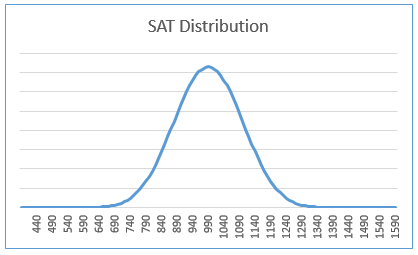
\includegraphics[width=\maxwidth{.95\linewidth}]{gfx/06-SATDistro}
	\caption{Normal Distribution}
	\label{fig06.01}
\end{figure}

SAT scores lie between $ 400 $ and $ 1600 $ as listed across the X-Axis and the number of students who earn each score is plotted. Since the most common score is $ 1000 $ that score is at the peak of the curve. Very few students scored above $ 1300 $ or below $ 650 $ and the curve is near the lower bound beyond those points. This illustrates a normal distribution where most scores are bunched near the center of the graph with only a few at either extreme.

The normal distribution is important because it permits researchers to use specific techniques to test a hypothesis about the sample. For example, perhaps a researcher hypothesized that the graduation rate at university ``A'' was higher than at university ``B'' because students' SAT scores were higher. Since SAT scores have a normal distribution, the researcher could use specific tests, like a t-test, to support or refute the hypothesis. However, if the data were not normally distributed then the researcher would need to use a different group of tests.

\subsection{Excess Kurtosis}
One way to mathematically describe a normal distribution is to calculate the length of the tails of a bell curve, and that is called its \gls{excesskurtosis}. For a normal distribution the excess kurtosis is $ 0.00 $, a positive excess kurtosis would indicate longer tails while a negative excess kurtosis would indicate shorter tails. Intuitively, many people believe the excess kurtosis represents the ``peaked-ness'' of the curve since longer tails would tend to lead to a more peaked graph; however, excess kurtosis is a measure of the data outliers, which would be only present in the tails of the graph; so excess kurtosis is not directly indicative of the the ``sharpness'' of the peak. It is difficult to categorically state that some level of excess kurtosis is good or bad. In some cases, data that form a graph with longer tails are desired but in other cases they would be a problem.

Following are three examples of excess kurtosis. Notice that as the excess kurtosis increases the tails become longer. 

\begin{figure}[H]
	\centering
	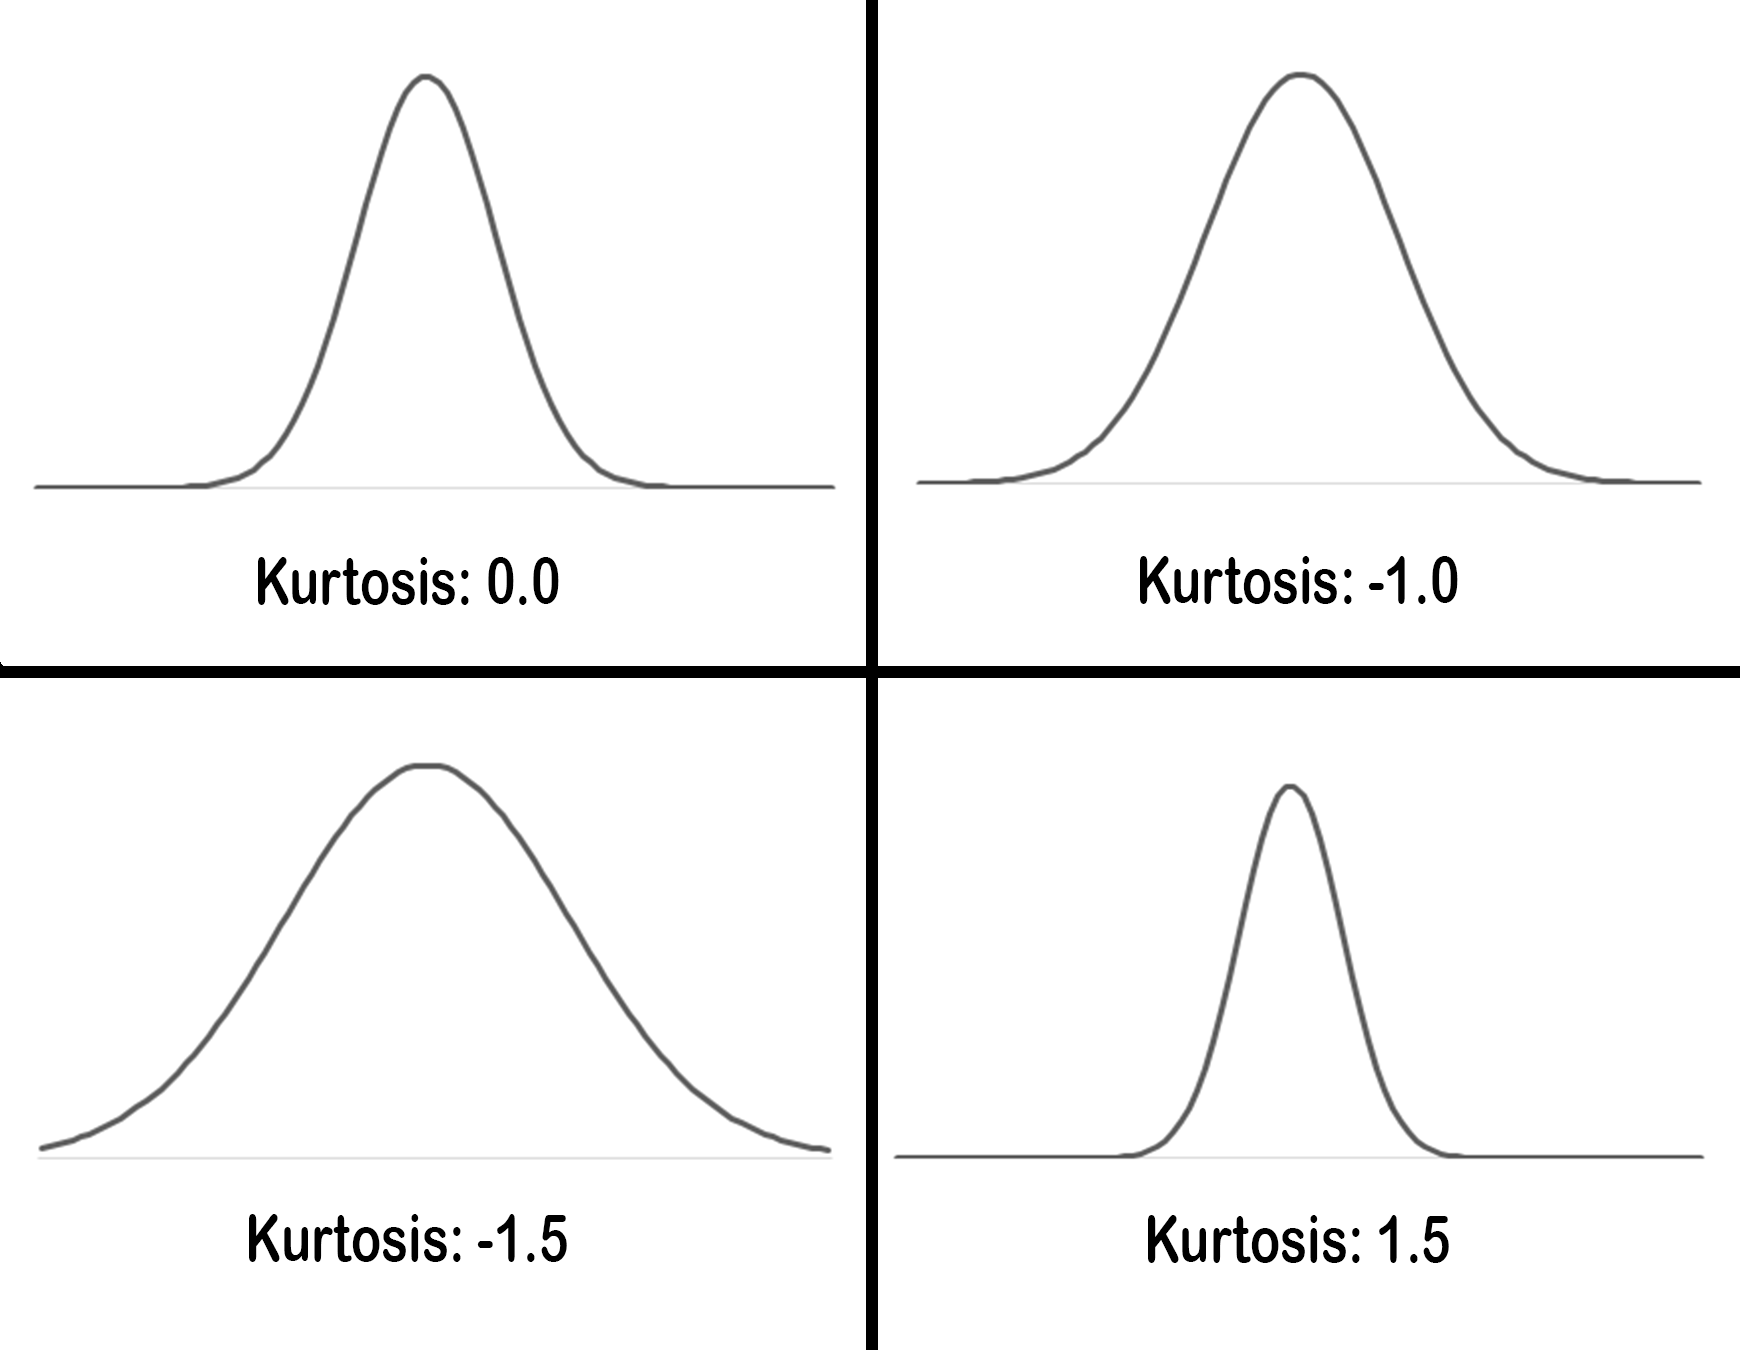
\includegraphics[width=\maxwidth{.95\linewidth}]{gfx/06-Kurtosis}
	\caption{Kurtosis in a Normal Distribution}
	\label{fig06.02}
\end{figure}

\subsection{Skew}
The second numerical measure of a normal distribution that is frequently reported is its \gls{skew}, which is a measure of the symmetry of the curve about the mean of the data. The normal distribution in Figure \ref{fig06.03} has a skew of $ 0.00 $. A positive skew indicates that the tail on the right side is longer, which means that there are several data points on the far right side of the graph ``pulling'' the tail out that direction. A negative skew indicates that the tail on the left side of the graph is longer. Following are three examples of skew:

\begin{figure}[H]
	\centering
	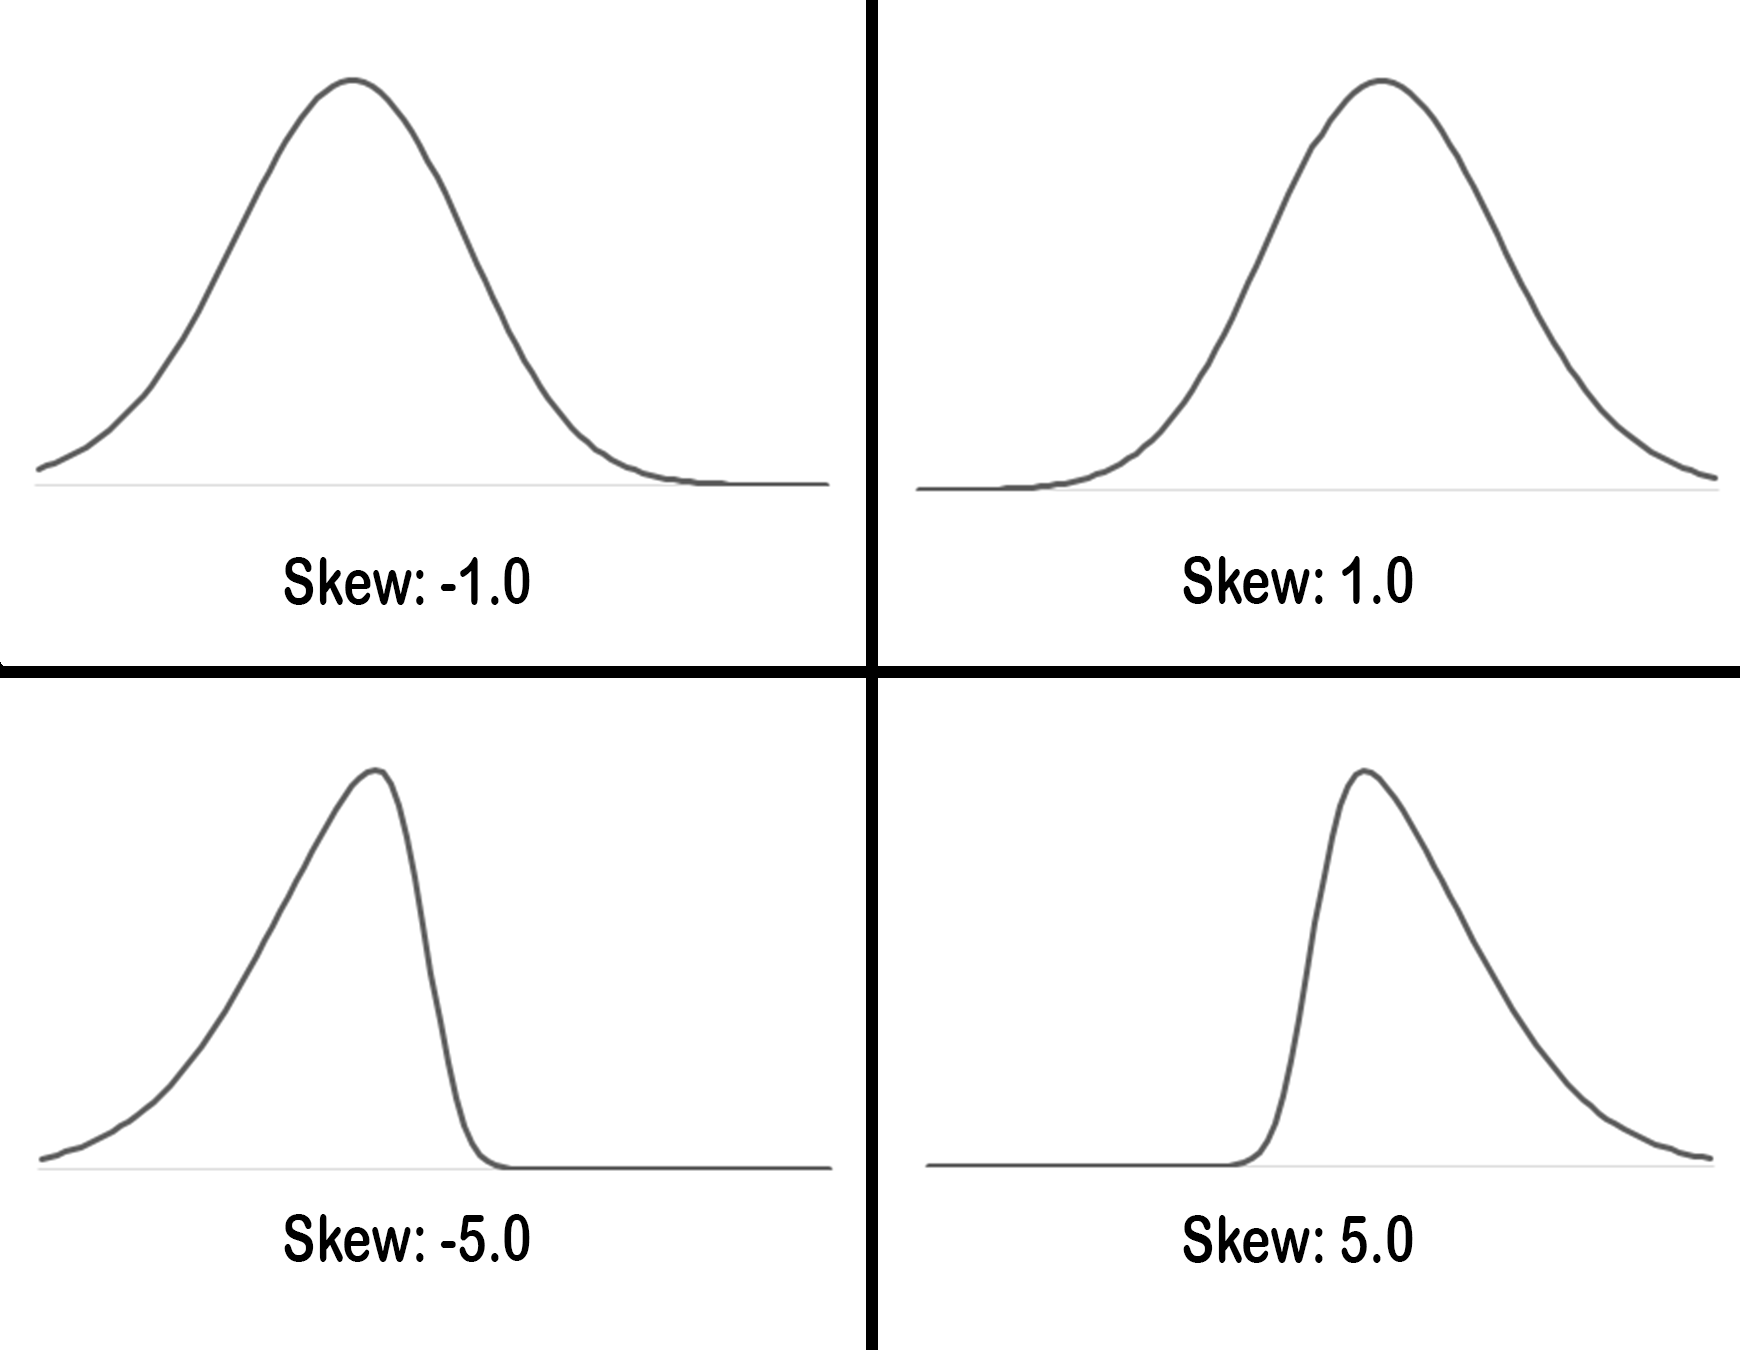
\includegraphics[width=\maxwidth{.95\linewidth}]{gfx/06-Skew}
	\caption{Skew in a Normal Distribution}
	\label{fig06.03}
\end{figure}

\section{Databases}

When a lot of data are gathered into a single location they are referred to as a \gls{database}. This is not a new concept. Fifty years ago a library would have a series of 3X5 cards that contained information about all of the books in the library (title, author, subject, etc.). Those cards were stored in a wooden cabinet called the ``card catalog'' and customers could find information about and the location of whatever book they wanted. Today, databases are often contained in electronic form on the internet where they can be accessed from customers' home computers, tablets, or even phones.

Data in a database is typically stored in tables that resemble spreadsheets, that is, rows and columns where each row is one record (or observation) about some phenomenon and each column is one descriptor of that record. For example, a database that contains information about the people who work at a company would be organized such that each row contained data about just one person and each column would contain a single aspect of that person's employment, like name, employee number, date of birth, etc.\footnote{Of course, databases are much more complex than described in this paragraph but this is not a database text so the simple explanation offered is adequate for this context.} A database is designed to deliver answers to questions through a lookup process so, for example, if the CEO of a company wanted to know the birth date for someone in the accounting department that data could be easily found. 

One common problem with any database is ``dirty data.'' These are data that contain errors or are missing. For example, it is easy for a data entry clerk to enter something like ``1000000'' instead of ``100000'' (count the zeros) for a person's salary and create an ``outlier'' in the data. Another common problem are missing data. For example, if employees are asked to update their personal information but someone could not remember their ZIP code then they would simply leave that field blank.

Dirty data makes it difficult to analyze the database. For example, if a researcher wanted to report the median salary for the workers in a factory but ten percent of the salaries were missing from the database then the median would not be accurate. There are several methods statisticians use to mitigate the problems caused by dirty data but those are beyond the scope of this text. 

\subsection{Public Databases}

There are hundreds of publicly available databases that can be used for research. As one example, the United States Census Bureau maintains a huge database that contains information about the people of the United States.\footnote{The US Census Bureau's website is at \url{https://www.census.gov/}.} The data at that site is freely available to anyone who wants to use it, and the site is organized so information is fairly quick and easy to find. As an example, it is not difficult to discover that among adults in the United States, 29\% have a high school diploma, 20\% have a Bachelor's degree, 8\% have a Master's degree, 1.7\% have a Doctoral degree, and the rest fall elsewhere on the education spectrum. The US Census Bureau has more advanced tools available that permit researchers to focus on a single county or even smaller region.

When using a public database, a researcher must be concerned with bias. Since the researcher did not gather the data first-hand it is possible that the data are biased. For example, if the database includes people's attitude towards work how is the researcher going to know if the data gathered was from a well-designed, neutral survey or if it was just gathered using some sort of convenience sample? In general, databases found at governmental websites (with urls that end with .gov) or education websites (with urls that end with .edu) would more likely be bias-free while databases from .com sites would need to have extra attention paid to bias.

Sometimes, students will find a website with a list of links to journal articles or chapters from books. While these are valuable resources for a researcher, they are not the same as a database that contains raw data from a survey, experiment, or other activity. Journal articles provide good information for a literature review but would not be appropriate for an online database source.

\subsection{Using Public Databases}

As an example of using a public database, imagine that the CEO of ``BASVFOODS'' is interested in opening a neighborhood market in a small town they have never serviced before. In order to gather information about that location it is possible to use US Census Bureau data to find out things like the median household size, income, and education level. The CEO could then compare that data with similar data from a town that has a successful store to help inform a decision to open a new store.

\section{Statistical Test Selection}

Once the data are gathered it is important to run appropriate statistical processes to see if the data contain anything of interest. There are hundreds of tests that can be used and researchers must consider both the goal of the analysis and the type of data being analyzed. The first step is to classify the variables being evaluated. 

\begin{itemize}
	\item \Gls{quantitativedata} are numeric and are generated through measurement or counting. \gls{continuousdata} can be any value, including fractions or decimals, like a person's height or the length of time it takes to complete some task. \Gls{discretedata} are integers normally found by counting, like the number of people at an event or the age of a respondent.
	\item \Gls{qualitativedata} are non-numeric and are often generated by people checking boxes on a survey. \Gls{ordinaldata} have some implied order, like a student's class (senior, junior, etc.) and \gls{nominaldata} have no order, like a respondent's gender.
\end{itemize}

\begin{figure}[H]
	\centering

	\forestset{qtree/.style={for tree={parent anchor=south, 
			child anchor=north,
			align=center,
			inner sep=3pt,
			draw}}}
		
	\begin{forest}, baseline, qtree
		[Variable, fill=purple!40!white
			[{Quantitative\\(Measure or count)}, fill=cyan!40!white
				[{Continuous\\(Any value)}, fill=cyan!20!white]
				[{Discrete\\(Integers)}, fill=cyan!20!white]
			]
			[{Qualitative\\(Tick boxes)}, fill=pink!60!white
				[{Ordinal\\(Ordered)}, fill=pink!40!white]
				[{Nominal\\(No order)}, fill=pink!40!white]
			]
		]
	\end{forest}

	\caption{Classifying Variables}
	\label{fig06.08}
\end{figure}

\subsection{Summary Statistics}

One of the easiest type of analysis to complete is determining the center and spread of a data set. This analysis is also one of the first that research readers expect to find. Here is a guide for what sort of central measure and spread to report.

\begin{itemize}
	\item For normally distributed continuous data use the mean and standard deviation.
	\item For skewed continuous or discrete data use the median and Interquartile Range (IQR).
	\item For ordinal data use the median and Interquartile Range (IQR).
	\item For nominal data use the mode as a central measure but there is no spread.
\end{itemize}

\begin{figure}[H]
	\centering
	
	\forestset{qtree/.style={for tree={parent anchor=south, 
				child anchor=north,
				align=center,
				inner sep=3pt,
				draw}}}
	
	\begin{forest}, baseline, qtree
		[Which summary and spread?, fill=brown!40!white
			[{Quantitative}, fill=orange!40!white
				[{Normal Distribution\\(Mean\\Standard deviation)}, fill=orange!20!white]
				[{Skewed Data\\(Median\\IQR)}, fill=orange!20!white]
			]
			[{Qualitative}, fill=yellow!60!white
				[{Ordinal\\(Median\\IQR)}, fill=yellow!40!white]
				[{Nominal\\(Mode\\No spread)}, fill=yellow!40!white]
			]
		]
	\end{forest}
	
	\caption{Central Measure and Spread}
	\label{fig06.09}
\end{figure}

\subsection{Parametric vs. Nonparametric Tests}

Normally, a researcher posits a hypothesis and then conducts research to either support or refute that hypothesis. The type of hypothesis test needed depends on the type of the variables being tested. There are two broad categories of variables in a hypothesis test: independent and dependent.

\begin{itemize}
	\item \Glspl{independentvariable} (explanatory variables) are those that cause something to happen; they explain why some outcome was observed. For example, if the hypothesis is that women spend more on groceries than men then the independent variable is the sex of the shopper. If the hypothesis is that old people are more dangerous drivers than young people then the independent variable is the age of the driver.
	\item \Glspl{dependentvariable} (outcome variables) are those that are the outcome for whatever is happening. For example, if the hypothesis is that women spend more on groceries than men then the dependent variable is amount of money spent. If the hypothesis is that elderly drivers are more dangerous than younger drivers then the dependent variable is the number of reported accidents.
\end{itemize}

The chart in Figure \ref{fig06.10} is used to determine if the hypothesis test should be parametric or nonparametric.

\begin{itemize}
	\item \Gls{parametric} tests assume that the data follow a particular distribution, usually normally distributed. Parametric tests are more powerful than nonparametric tests and are more likely to detect true differences or relationships that exist.
	\item \Gls{nonparametric} tests are used when the dependent variable is not normally distributed; that is, the data are skewed or are qualitative. Nonparametric techniques are usually based on ranks or signs rather than the actual data and are usually less powerful than parametric tests.
	\item \Gls{chisquare} is a test that is only used when the dependent variable is nominal in nature. A chi-square test determines if there is a significant difference in the actual observed frequencies and those hypothetically expected. For example, if a coin were tossed $ 100 $ times it would be expected to land ``heads'' half of the time but if the actual observation was that ``heads'' came up $ 75\% $ of the time then the chi-square statistic would indicate that this was a significant difference.
\end{itemize}

\begin{figure}[H]
	\centering
	
	\forestset{qtree/.style={for tree={parent anchor=south, 
				child anchor=north,
				align=center,
				inner sep=3pt,
				draw}}}
	
	\begin{forest}, baseline, qtree
		[Dependent Variable, fill=green!40!white
		[{Quantitative}, fill=teal!40!white
		[{Normal Distribution\\(Parametric)}, fill=teal!20!white]
		[{Skewed Data\\(Nonparametric)}, fill=teal!20!white]
		]
		[{Qualitative}, fill=lime!60!white
		[{Ordinal\\(Nonparametric)}, fill=lime!40!white]
		[{Nominal\\(Chi-square)}, fill=lime!40!white]
		]
		]
	\end{forest}
	
	\caption{Parametric vs. Nonparametric Selection}
	\label{fig06.10}
\end{figure}

\subsection{Hypothesis Test Selection}

Researchers often hypothesize\footcite{Chapter \ref{ch14:mixed} contains more information about hypothesis testing.} that some treatment will lead to an outcome. In order to test that, they will apply the treatment to one group but not another and then compare the two groups to see if there is any difference. Table \ref{tab06.07} lists the statistical tests that are commonly used to compare the averages of two or more groups. In the table, ``independent'' groups are those that have no overlapping members while ``matched'' groups test the same members two times. As an example, if researchers wanted to know how if a movie affected people in some way they could survey people leaving two different theaters (independent groups) or survey the same people before and after seeing the movie (matched groups).

\begin{table}[H]
	\centering
	\definecolor{ltgray}{gray}{0.95} % this is a light gray
	\rowcolors{1}{}{ltgray} % zebra striping background
	\begin{tabularx}{0.95\linewidth}{p{0.25\linewidth}
			p{0.15\linewidth}
			p{0.15\linewidth}
			p{0.15\linewidth}
			p{0.15\linewidth}
		}
		\toprule
		\textbf{Comparing} & 
			\textbf{Dep Var} & 
			\textbf{Ind Var} &
			\textbf{Para} & 
			\textbf{NonPara} \\
		\midrule
		2 independent \newline groups & Quant & Binary & Indep t-test & Mann-Whitney \\
		3+ independent \newline groups & Quant & Nom & ANOVA & Kruskal-Wallis \\
		2 matched \newline groups & Quant & Time & Paired t-test & Wilcoxon \\	
		3+ measures \newline same subj & Quant & Time & Rep ANOVA & Friedman \\		

		\bottomrule
	\end{tabularx}
	\caption{Tests to Compare Two or More Samples}
	\label{tab06.07}
\end{table}

Another common research goal is to see if there is any association (or ``correlation'') between two or more variables. Further, a correlation may be able to predict an outcome for a new observation. For example, a researcher may run an experiment where students work with a tutor once a week and then see if there is an improvement in test scores. In this case, ``tutoring time'' would be correlated with ``test scores'' and that may be used to predict a new student's test score based on the amount of tutoring time. Table \ref{tab06.08} lists the hypothesis tests that are commonly used to find correlations and predictions between two groups.

\begin{table}[H]
	\centering
	\definecolor{ltgray}{gray}{0.95} % this is a light gray
	\rowcolors{1}{}{ltgray} % zebra striping background
	\begin{tabularx}{0.95\linewidth}{p{0.25\linewidth}
			p{0.15\linewidth}
			p{0.15\linewidth}
			p{0.15\linewidth}
			p{0.15\linewidth}
		}
		\toprule
		\textbf{Comparing} & 
		\textbf{Dep Var} & 
		\textbf{Ind Var} &
		\textbf{Para} & 
		\textbf{NonPara} \\
		\midrule
		2 Continuous & Quant & Quant & Pearson's r & Spearman's rho \\
		Prediction & Quant & Any & Regression & None \\
		Prediction & Nominal & Any & Log \newline regression & None \\	
		2 Qual vars & Qual & Qual & None & Chi-square \\		
		
		\bottomrule
	\end{tabularx}
	\caption{Tests to Association Between Two Samples}
	\label{tab06.08}
\end{table}


\section{Statistical Test Sampler}

While there are hundreds of statistical procedures available, this section covers those that are commonly used.

\subsection{Central Measures}

Three different central measures are commonly used, depending on the type of data being summarized.

\begin{itemize}
	\item \textbf{Mean}. An arithmetic mean is calculated by adding together all of the terms and then dividing by the number of terms. This process is taught in elementary school as calculating the ``average.'' However, if the terms have wildly different values then a \textit{geometric mean} is a better choice. In a geometric mean the values are multiplied together and then the n-root is taken, where ``n'' is the number of terms in the data. Finally, if the mean of a series of rates is needed, then a \textit{harmonic mean} is used. For a harmonic mean all of the terms are reciprocated, a mean is found of those reciprocated terms, and then the mean is reciprocated.
	\item \textbf{Median}. A median is found by putting all of the terms in numeric order and then selecting the middle term. This is useful if the data set includes outliers, that is, a few values far outside the other terms. Medians are frequently used to report house values since a few houses may be worth far more than the other houses in an area. If the data set has an even number of terms, so there is no middle term, then the median is found by taking the mean of the middle two terms.
	\item \textbf{Mode}. The mode is used for nominal data and is the count of the most common term. For example, if a count of the number of undergraduate students in each class (senior, junior, etc.) is made and it turns out that there are more seniors than any other group then the mode would be ``senior.''
\end{itemize}

\subsection{Spread}

Two measures of spread are commonly used. 

\begin{itemize}
	\item \textbf{Range}. The range, or ``dispersion,'' is the difference between the highest value and lowest value.
	\item \textbf{Standard deviation}. This often misunderstood value is nothing more than an indicator of how much variation exists in the data, or how ``scattered out'' the data are. In general, the greater the standard deviation the more variation there are in the data. As an example, imagine that a professor administered an examination to a group of students and found the mean to be $ 70\% $ with a standard deviation of $ 15 $. Then the professor changed something about the class the next semester and administered the same examination to that group of students and found the mean was $ 85\% $ with a standard deviation of $ 5 $. This result would indicate that the scores the second semester had much less variation, they were much ``tighter,'' and that would likely be good news for the professor.
\end{itemize}

\subsection{Frequency Tables}

Discrete or qualitative data items are normally reported in frequency tables where the counts for a particular item are displayed. When a frequency table has two dimensions it is usually called a ``cross-tab'' or ``pivot table.'' As an example, Table \ref{tab06.02} contains the results of an exit poll from 2016 presidential election. \cite{cnn2016election}

\begin{table}[H]
	\centering
	\definecolor{ltgray}{gray}{0.95} % this is a light gray
	\rowcolors{1}{}{ltgray} % zebra striping background
	\begin{tabularx}{0.95\linewidth}{
			p{0.22\linewidth}
			p{0.22\linewidth}
			p{0.22\linewidth}
			p{0.22\linewidth}}
		\toprule
		\textbf{Party} & \textbf{Clinton} & \textbf{Trump} & \textbf{Other} \\
		\midrule
		Democrats & $ 89\% $ & $ 8\% $ & $ 3\% $ \\
		Republicans & $ 8\% $ & $ 88\% $ & $ 4\% $ \\
		Independents & $ 42\% $ & $ 46\% $ & $ 12\% $ \\
		\bottomrule
	\end{tabularx}
	\caption{2016 Exit Poll.}
	\label{tab06.02}
\end{table}

\subsection{Correlation}

\Gls{correlation} is a method used to describe a relationship between the independent (or x-axis) and dependent (or y-axis) variables in a research project. A correlation is expressed as a number between $ -1.0 $ and $ +1.0 $ where the closer the correlation gets to the extremes the more meaningful it becomes. Thus, two variables with a correlation of $ +0.65 $ have a closer association than two variables with a correlation of $ +0.23 $. Correlations are often displayed in a matrix. Table \ref{tab06.06} shows the Miles per Gallon, Displacement, and Horsepower for a group of automobiles. In this table, notice that there is a negative correlation between horsepower and miles per gallon, which means that cars with greater horsepower get fewer miles per gallon. On the other hand, there is a positive correlation between displacement and horsepower so cars with greater engine displacement have more horsepower.

\begin{table}[H]
	\centering
	\definecolor{ltgray}{gray}{0.95} % this is a light gray
	\rowcolors{1}{}{ltgray} % zebra striping background
	\begin{tabularx}{0.95\linewidth}{
			p{0.22\linewidth}
			p{0.22\linewidth}
			p{0.22\linewidth}
			p{0.22\linewidth}}
		\toprule
		{}   & mpg       & disp      & hp \\
		mpg  & $ +1.00 $ & $ -0.85 $ & $ -0.78 $ \\
		disp & $ -0.85 $ & $ +1.00 $ & $ +0.79 $ \\
		hp   & $ -0.78 $ & $ +0.79 $ & $ +1.00 $ \\
		\bottomrule
	\end{tabularx}
	\caption{Selected Automobile Correlations.}
	\label{tab06.06}
\end{table}


\subsection{Parametric Hypothesis Tests}

Some analysis techniques are only useful with \gls{parametric} data. While there are dozens of statistical processes that will work with parametric data, two are most commonly seen.

\begin{itemize}
	\item \textbf{\Gls{ttest}}. A t-test is used to analyze the difference in two groups of samples that are normally distributed. For example, a researcher may hypothesize that there is a significant difference in the ages of people in two towns. Once people's ages are recorded a t-test could be used to see if there is a significant difference in the mean age for the people in those two towns.
	
	There are two varieties of t-test commonly used, depending on the type of data being analyzed. If the two groups being compared are independent of each other then an ``independent t-test'' would be used. However, researchers often use the same group but test them at two different times. For example, a medical trial may measure some factor (like blood presure), apply some treatment, and then measure the factor a second time. In that case, a ``paired t-test'' would be used where the values from the first trial would be compared to those in the second.
	
	\item \textbf{Analysis of Variance (ANOVA)}. An \Gls{anova} is similar to a t-test but is used to analyze three or more groups to see if there is a significant difference in any of the groups.
\end{itemize}

The result of either a t-test or ANOVA is a \textit{p-value} (``probability value''). A p-value describes the probability that some result was caused by pure chance and not from some applied treatment. P-values are expressed as percentages and, normally, researchers expect a p-value under $ 0.05 $ ($ 5\% $) in order to declare the result to be significant. If the calculated p-value is above $ 0.05 $ then the researcher declares that no significant result was found.

\subsection{Nonparametric Hypothesis Tests}

Some analysis techniques are only useful with \gls{nonparametric} data. While there are dozens of statistical processes that will work with nonparametric data, two are most commonly seen.

\begin{itemize}
	\item \textbf{Mann-Whitney U}. This test is used to determine if there are any significant differences in two groups of data that are not normally-distributed, often categorical. As an example of using a Mann-Whitney U test, Gluck et al. used it in \textit{How Short Is Too Short? Implications of Length and Framing on the Effectiveness of Privacy Notices}\cite{gluck2016short}. This study postulated that privacy notices were so long people did not often read, or understand, them. They conducted an experiment where they presented groups of people with both short and long privacy notices and then assessed their understanding. A Mann-Whitney U test was used to compare the groups and, not surprisingly, people who used the short form seemed to understand their privacy rights better than those who used a long form. This experiment also varied the framing of the policy (positive vs. negative) and used a Kruskal-Wallis H test to compare the results but they found no effect provided by different framing. This study is a good example of using both Kruskal-Wallis H and Mann-Whitney U in a single analysis.
	
	\item \textbf{Kruskal-Wallis H}. This test is used to determine if there are any significant differences in three or more groups of data that are not normally-distributed, often categorical. As an example of using a Kruskal-Wallis H test, Titlebaum and Lawrence published \textit{Perceived Motivations for Corporate Suite Ownership in the ``Big Four'' Leagues}\cite{titlebaum2016perceived}. This study looked at $ 29 $ different reasons (entertain clients, support the community, and business-to-business networking, etc.) corporations purchase luxury suites in any of the four major sports leagues (NFL, MLB, NBA, and NHL). They surveyed corporate leadership and then applied a Kruskal-Wallis H test to the survey results to see which reason was most important. They found four that were significant: 1) Entertaining Employees, 2) Supporting the Community, 3) Perception of the Company in the Community, and 4) Customized Gifts for Suite Owners. They also compared the leagues, two at a time, to see if the reasons were different between the leagues and used a Mann-Whitney U test for this part of the analysis. They found that MLB had a significantly higher rank for ``Entertaining Employees'' than all of the other sports. This study is a good example of using both Kruskal-Wallis H and Mann-Whitney U in a single analysis.
\end{itemize}

The result of either a Mann-Whitney U or Kruskal-Wallis H is a \gls{pvalue} (``probability value''). A p-value describes the probability that some result was caused by pure chance and not from some applied treatment. P-values are expressed as percentages and, normally, researchers expect a p-value under $ 0.05 $ ($ 5\% $) in order to declare the result to be significant. If the calculated p-value is above $ 0.05 $ then the researcher declares that no significant result was found.

\section{Data Mining}

Data mining is a relatively new statistical technique that attempts to extract (``mine'') valuable intelligence from massive databases. Raval\cite{raval2012data} published an excellent overview of data mining techniques. As but one example, a grocery store chain mines customer purchases, shopping habits, and other data to plan sales, send coupons, and make other suggestions that will, hopefully, lead to increased spending. While there are more than a dozen data mining techniques, these three are most common.

\subsubsection{Clustering}

It is beneficial to ``cluster'' customers in some way so advertising (and sales) can be more effective. For example, if a large grocery store chain can determine that most of the customers in one region share some common trait then it becomes easier to market to that region.

Figure \ref{fig06.11} shows a scatter plot with three clusters. This plot was generated from dummy data but it shows the type of clustering that a researcher may be able to find in a data set. The location of a specific cluster in relationship to the others would perhaps drive a marketing campaign focused on the specific properties the customers in that one cluster share.

\begin{figure}[H]
	\centering
	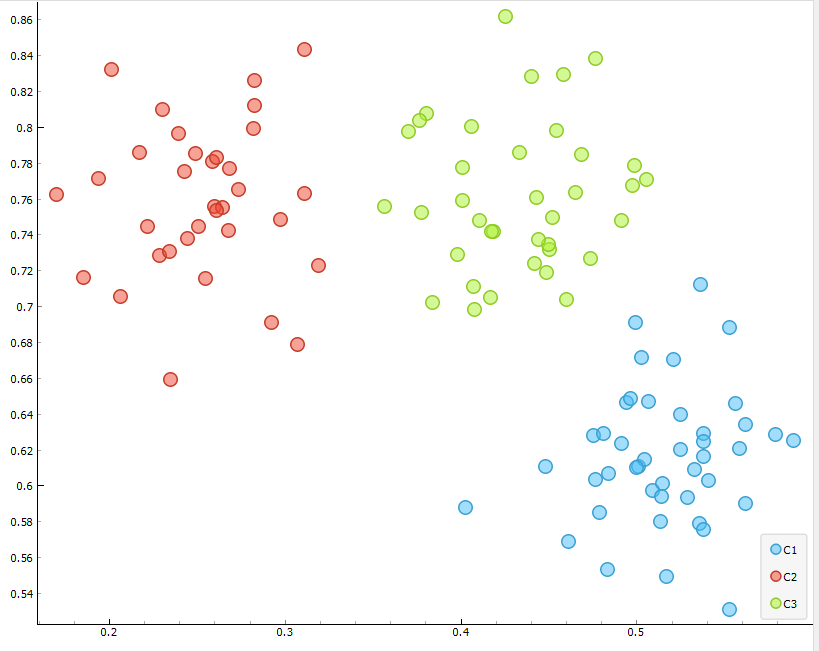
\includegraphics[width=\maxwidth{.95\linewidth}]{gfx/06-Cluster}
	\caption{Example of Clustering}
	\label{fig06.11}
\end{figure}

As an example of using clustering, Vogel, Greiser, and Mattfeld publised \textit{Understanding Bike-Sharing Systems using Data Mining: Exploring Activity Patterns}\cite{vogel2011understanding} in 2011. They analyzed more than $ 760,000 $ pickups and returns at bike stations in Vienna from $ 2008-2009 $. Their goal was to determine if the stations could be clustered in some way by usage patterns. They used cluster analysis to divide the city's stations into five groups, for example, the ``returns morning pickups evening'' group showed especially high number of morning returns and evening pickups. They provided the city with information that was designed to help in future station placement.

\subsubsection{Decision Tree}

A decision tree organizes known data so predictions can be made on new data. Figure \ref{fig06.05} is taken from a data set that shows the fate of all the passengers on the Titanic. Starting at the top, few males survived. Of the females, there were no survivors who had more than $ 4.5 $ siblings or spouses on board, so large families perished. Notice, though, that near the bottom of the tree nearly all first class female passengers with few family members on board survived. A decision tree like this could be used to predict whether a given passenger survived. 

\begin{figure}[H]
	\centering
	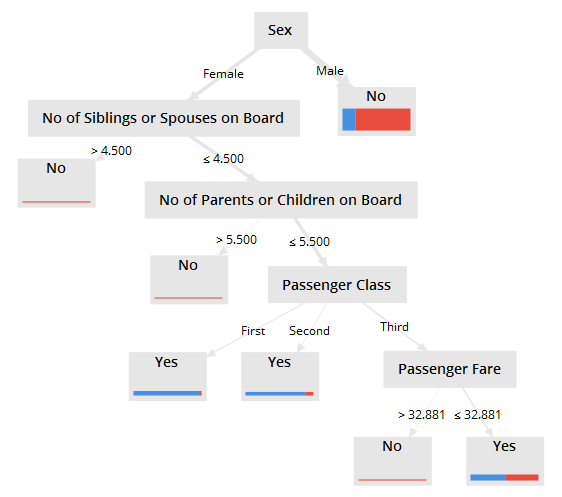
\includegraphics[width=\maxwidth{.95\linewidth}]{gfx/06-DecisionTree}
	\caption{Decision Tree}
	\label{fig06.05}
\end{figure}

As an example of using a decision tree, Ona, Ona and Lopez completed a study of the Grenada, Spain, public transportation system\cite{de2016transit}. They data mined $ 3,664 $ passenger surveys conducted from $ 2008 $ until $ 2011 $. The surveys asked passengers some demographic questions (age, etc.) and about various aspects of the bus service. The researchers first created four clusters of passenger types using cluster analysis, ``Young Students,'' ``Working Women,'' ``Sporadic Users,'' and ``Elderly Passengers.'' Then they generated five different decision trees, one for each group and one overall, to define the difference between ``poor'' and ``good'' service ratings from the passengers. For example, in the Overall tree, service frequency was the first, most important, branch on the tree; but for Young Students the first branch was punctuality. This is an excellent study that is easy to read and understand and shows how two different data mining techniques, cluster analysis and decision tree building, can be used in a single study.

\subsubsection{Market Basket}

A market basket analysis evaluates the products that customers purchase at the same time (they are in the same ``market basket'') and then uses that data to drive decisions on things like store organization and sales. For example, it is well known that customers who purchase beer also tend to purchase potato chips. What may be surprising is that customers who purchase beer also tend to purchase baby diapers. A market basket analysis does not attempt to determine why these relationships exist, just that they do exist. A grocery store owner may chose to put beer and chips on sale at the same time or create a display near the front of the store with both beer and chips. 

Figure \ref{fig06.06} is a graphic representation of the rule set found in Figure \ref{fig06.10}, created from a market basket analysis of a bakery. The goal was to determine what sorts of products customers purchased with cherry tarts. Rule $ 53 $ indicates that apricot danish and cherry tarts tend to be purchased at the same time, and that would be valuable information for a bakery owner. The explanation of the numbers displayed (``Support,'' ``Confidence,'' etc.) is beyond the scope of this class, but business owners would want to work with a researcher who could complete this sort of analysis.

\begin{figure}[H]
	\centering
	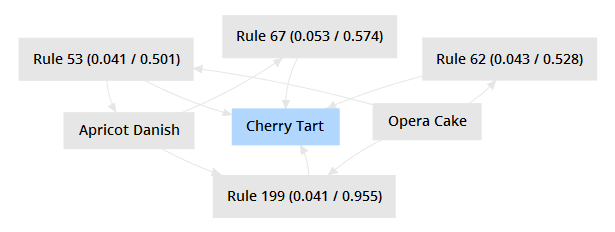
\includegraphics[width=\maxwidth{.95\linewidth}]{gfx/06-MarketBasketGraph}
	\caption{Market Basket Graph}
	\label{fig06.06}
\end{figure}


\begin{figure}[H]
	\centering
	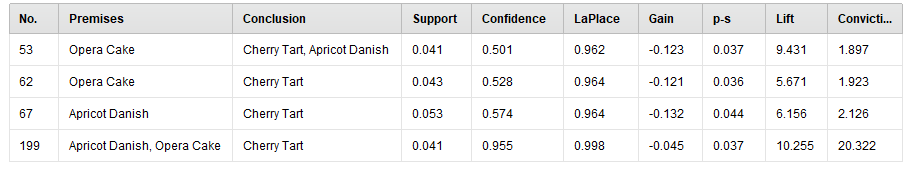
\includegraphics[width=\maxwidth{.95\linewidth}]{gfx/06-MarketBasketRules}
	\caption{Market Basket Rules}
	\label{fig06.07}
\end{figure}

As an example of a market basket analysis, Musalem, Aburto, and Bosch completed a study of a mid-sized supermarket in Latin America\cite{musalem2018market}. That market sells approximately $ 7,000 $ products and the average basket size is products from $ 3.6 $ categories. They reviewed the register receipts from the month of July 2000 and recorded the products sold, units sold, date, and time. They categorized the products into four categories: non-perishable (cereals, flour, noodles, etc.), immediate consumption (meat, milk, cheese, etc.), hygiene (shampoo, conditioner, diapers, etc.), and hedonic (ice cream, beer, candy, etc.). They found that items in the hygiene basket were associated with larger transactions but there were not many of them. The non-perishable basket had a high number of different categories and a high transaction size, so these buyers are extremely important to the market. This study is a good example of how market basket analysis can be used to improve sales.

\section{Summary}\label{ch06:summary}

Figure \ref{fig06.04} illustrates the relationship between the various types of data and the rating scales commonly used to work with those data types. Researchers with a positivism philosophy tend to use parametric statistical analysis and gather interval and ratio data. Researchers with an interpretivism philosophy tend to use nonparametric statistical analysis and gather nominal and ordinal data. Nominal data are typically gathered with binary and semantic difference rating scales while ordinal data are typically gathered with Likert and Guttman rating scales.

\begin{figure}[H]
	\centering
	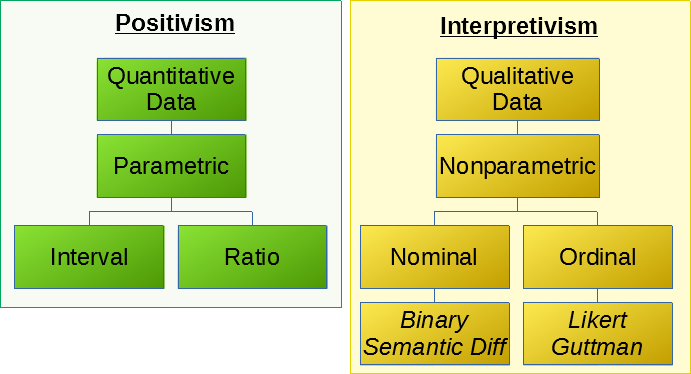
\includegraphics[width=\maxwidth{.95\linewidth}]{gfx/06-DataTypes}
	\caption{Data types}
	\label{fig06.04}
\end{figure}
